\documentclass[10pt,a4paper]{report}
\usepackage[utf8]{inputenc}
\usepackage[german]{babel}
\usepackage[T1]{fontenc}
\usepackage{amsmath}
\usepackage{amsfonts}
\usepackage{amssymb}
\usepackage{graphicx}
\author{Julian Sobott (76011), David Sugar (76050), Lukas Mendel (76009)}
\title{Bericht Datenbank Praktikum}
\begin{document}
\maketitle
\tableofcontents

\newpage
\section{Aufgabe 1}
\subsection{a)}
\begin{figure}[h]
	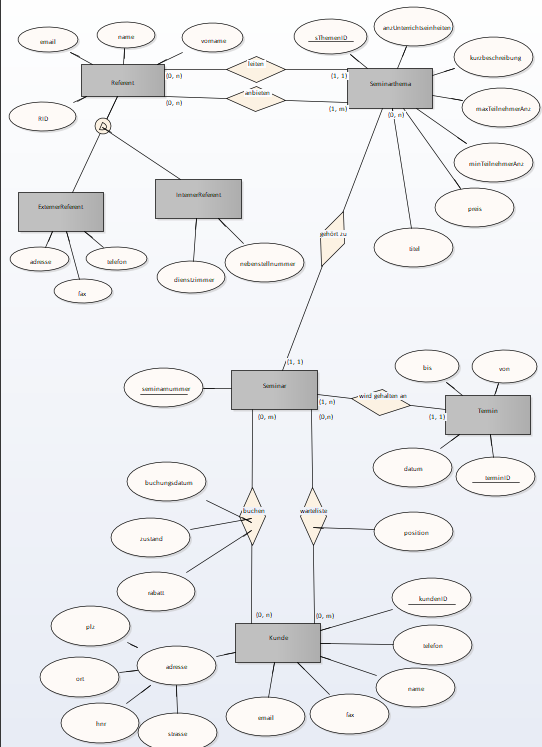
\includegraphics[scale=0.7]{Bilder/ER-Modell.PNG}
	\caption{ER-Modell Seminarverwaltung}
	\label{er:1}
\end{figure}

\subsubsection{Entities}
seminar = (\{\underline{SEMINARNUMMER:STRING}\})

termin  = (\{\underline{TERMINID:STRING}, DATUM:DATE, VON:DATETIME, BIS:DATETIME\})

kunde   = (\{\underline{KUNDENID:STRING}\})

\subsubsection{Relations}

\subsection{b)}

\end{document}